\section{Wechselwirkende Teilchen}
\begin{tabbing}
\hspace{4em} \= \hspace{4em} \= \kill
Mögliche Syteme beziehungsweise Lösungen\\
(1)\> Schwache Wechselwirkung $\rightarrow$ Störungstheorie für Zustandssumme\\
\> $ Z = \frac{1}{N!}\int \frac{1}{h^{3N}}\exp \left(-\beta\left[\sum_j \frac{\vec{p}^2_j}{2 m} + \frac{1}{2} \sum_{j,l}u\left(\vec{r}_j - \vec{r}_l\right)\right]\right)\dd{}^3 p_1\dots \dd{}^3 p_N \dd{}^3 r_1\dots \dd{}^3 r_N$\\
\> $u \vcentcolon  = \frac{1}{2} \sum_{j,l}u\left(\vec{r}_j - \vec{r}_l\right)$\\
\> $e^{-\beta u} \approx 1 - \beta u + \frac{1}{2} \beta^2 u^2 + \dots$\\
(2)\> Mean-Field-Theorie\\
\> Ersetze $U\left(\vec{r}_1, \dots, \vec{r}_N\right) = \sum\limits_j u_{eff} \left(\vec{r}_j\right)$ mit effektivem Potential $u_{eff}$\\
(3)\> Neue Koordinaten, so dass ungekoppelte Freiheitsgrade (Normalmoden).\\
\> $\rightarrow$ Nichtwechselwirkendes Gas\\
\>Beispiel: Phononengas, siehe Übung\\
(4)\> Exakte Lösung, zum Beispiel Ising-Modell (wechselwirkende Spins)
\end{tabbing}


\subsection{Mean-Field-Theorie (Molekularfeldnäherung): van der Waals-Gas}
\begin{tabbing}
\hspace{4em} \= \hspace{4em} \= \kill
Betrachte nicht-ideales klassisches Gas, Hamiltonfunktion:\\
\> $H = \frac{1}{2 m} \sum\limits_j \vec{p}_j^2 + u$\\
\> $U = \frac{1}{2}\sum\limits_{j,l} u\left(\left|\vec{r}_j - \vec{r}_l\right|\right)$\\
Zum Beispiel Lennard-Jones-Potential: $u(r) = u_0 \left[\left(\frac{r_0}{r}\right)^{12} - 2 \left(\frac{r_0}{r}\right)^6\right]$\\
\> Term $-2 \left(\frac{r_0}{r}\right)^6$: van der Waals-Anziehung\\
Einfacher: Hardcore-Potential
\end{tabbing}
\begin{figure}[H]
  \centering
  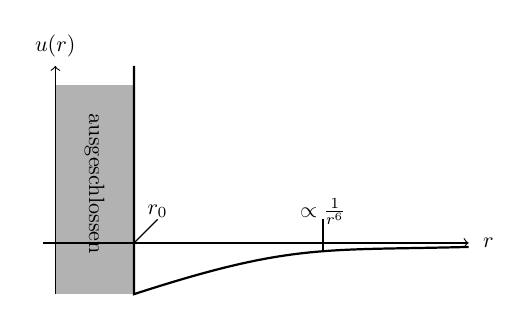
\begin{tikzpicture}[every node/.style = {draw = none, fill = none,scale = 0.8}]
    \path[draw=none,fill=white!70!black] (0,-0.65) to (0,2) to (1,2) to (1,-0.65);
    \draw[->] (0,-0.65) to (0,2.25);
    \draw[->] (-0.15,0) to (5.25,0);
    \node at (0,2.5) {$u(r)$};
    \node at (5.5,0) {$r$};
    \draw[thick] (1,2.25) to (1,-0.65) .. controls (3,0) and (3.4,-0.1) .. (5.25,-0.05);
    \draw (1,0) to (1.3,0.3);
    \path (0.5,2) to node[sloped] {ausgeschlossen} (0.5,-0.5);
    \node at (1.3,0.4) {$r_0$};
    \draw (3.4,-0.1) to (3.4,0.3);
    \node at (3.4,0.4) {$\propto \frac{1}{r^6}$};
  \end{tikzpicture}
  \\
  $u(r) = \left\{ \begin{array}{r@{\quad : \quad} l}\infty & r < r_0 \\ -u_0 \left(\frac{r_0}{r}\right) & r > r_0\end{array}\right.$
\end{figure}
\begin{tabbing}
\hspace{4em} \= \hspace{4em} \= \kill
$Z$\> $= \frac{1}{N!}\int \frac{1}{h^{3N}}\exp \left(-\beta\left[\sum_j \frac{\vec{p}^2_j}{2 m} + \frac{1}{2} \sum_{j,l}u\left(\left|\vec{r}_j - \vec{r}_l\right|\right)\right]\right)\dd{}^3 p_1\dots \dd{}^3 p_N \dd{}^3 r_1\dots \dd{}^3 r_N$\\
\> $= \frac{1}{N!}\frac{1}{\Lambda^{3N}}\int\dd{}^3r_1\dots\dd{}^3r_N e^{-\beta u}$ (kanonische Zustandssumme)\\
mit $\Lambda = \frac{h}{\sqrt{2\pi m k_B T}}$\\
Mean-Field: $u \rightarrow \sum\limits_j u_{eff}\left(\vec{r}_j\right)$\\
$\rightarrow$\> $Z = \frac{1}{N!}\frac{1}{\Lambda^{3N}}\left[\int \dd{}^3r e^{-\beta u_{eff}\left(\vec{r}\right)}\right]^N$\\
Schätzung des Integrals: $\approx (V - V_{ex})e^{-\beta \bar{u}_{eff}}$\\
Schätzung des ausgeschlossenen Volumens $V_{ex}$:\\
\> Sei $r_0 = $ kleinstmöglicher Abstand; $v_0 = \frac{4}{3}\pi r_0^3$\\
\> 1. Teilchen: ausgeschlossen: $\Delta V_{ex} = 0$\\
\> 2. Teilchen: ausgeschlossen: $\Delta V_{ex} = v_0$\\
\> 3. Teilchen: ausgeschlossen: $\Delta V_{ex} = 2 v_0$\\
$\rightarrow$\> $V_{ex} = \frac{1}{N} \cdot \left(0+v_0 + 2 v_0 + \dots + (N-1) v_0\right) = \frac{1}{N}v_0 \cdot \frac{N}{2} (N - 1) = \frac{(N-1) v_0}{2}$\\
$N-1 \approx N$\\
$\rightarrow$\> $V_{ex} = N \frac{v_0}{2} = \vcentcolon N b$ $b =$\glqq\underline{Kovolumen}\grqq\\
Schätzung für $\bar{u}_{eff}$: Betrachte zunächst $\bar{u}$ für zwei herausgegriffene Teilchen,\\
\> $\bar{u} = \int\limits_{0}^{\infty} u(r) \frac{4\pi r^2}{V} \dd{r} = - u_0\frac{4\pi}{V} \int\limits_{r_0}^{\infty} \frac{r_0^6}{r^4}\dd{r} = -\frac{u_0}{V}\frac{4}{3}\pi r_0^3 = - u_0 \frac{v_0}{V}$\\
\> Wobei $\frac{4\pi r^2}{V} \dd{r}$ die Wahrscheinlichkeit ist, das zweite Teilchen in $\dd{r}$ zu finden.\\
\> Gesamte potentielle Energie: $U ={N \choose 2} \bar{u} \approx \frac{N^2}{2} \bar{u}$\\
\> $U \stackrel{!}{=} N \bar{u}_{eff}$ $\rightarrow$ $\bar{u}_{eff} = \frac{N}{2} \bar{u} = - \frac{N}{V} u_0 v_0 = \vcentcolon -\frac{N}{V}a$\\
\> mit \underline{Kohäsionsparameter} $a$\\
$\rightarrow$\> $\int\dd{}^3r e^{-\beta \bar{u}_{eff}} \approx (V - N b) e^{\beta N a /V}$ $\rightarrow$ \fbox{$Z = \frac{1}{N!}\frac{(V - N b)^N}{\Lambda^{3N}}e^{\beta N^2 a / V}$}\\
Herleitung der thermischen Zustandsgleichung:\\
\> $\dd{F} = - S \dd{T}-p\dd{V} + \mu\dd{N}$\\
$\rightarrow$\> $p = -\left(\frac{\partial F}{\partial V}\right)_{T,N} = - \left(\frac{\partial}{\partial V}\right)_{T,N}(-k_B T \ln Z)$\\
\> $ = k_B T \frac{\partial}{\partial V} \ln \left[(V - N b)^N e^{\beta N^2 a / V}\right] = k_B T \left[\frac{N}{V - N b} - \frac{N^2 a}{V^2 k_B T}\right]$\\
$\rightarrow$\> \fbox{$\left(p + a\frac{N^2}{V^2}\right)\cdot (V - N b) = N k_B T$} (\underline{van der Waals-Zustandsgleichung})\\
Ideales Gas $\rightarrow$ van der Waals-Gas:\\
\> $p_{\text{ideal}} \stackrel{\wedge}{=} p + a \frac{N^2}{V^2}$, Druck ist durch attraktive Wechselwirkung verringert ($p < p_{\text{ideal}}$)\\
\> $V_{\text{ideal}} \stackrel{\wedge}{=} V - N b$, Gas nimmt wegen des Eigenvolumens der Teilchen mehr Raum ein ($V > V_{\text{ideal}}$)\\
\underline{Isothermen}:\\
In der Nähe von $-\left(\frac{\partial p}{\partial V}\right)_T < 0$ ist der Zustand instabil und geht in die Koexistenz zweier Phasen\\
(flüssig, gasförmig) über
\end{tabbing}
\begin{figure}[H]
  \centering
  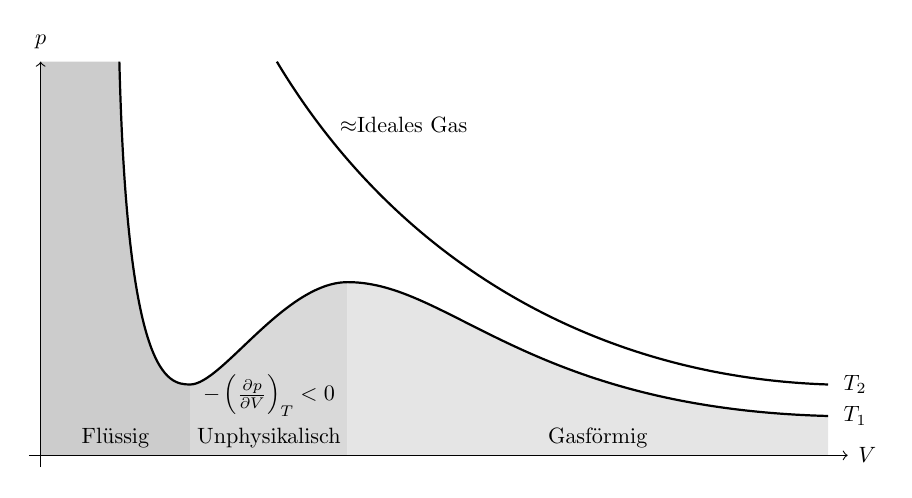
\begin{tikzpicture}[every node/.style = {draw = none, fill = none,scale = 0.8}]
    \path[fill=white!80!black] (0,5) to (1,5) .. controls (1.1,1) and (1.6,0.9) .. (1.9,0.9) to (1.9,0) to (0,0);
    \path[fill=white!85!black] (1.9,0) to (1.9,0.9) .. controls (2.3,0.9) and (3.1,2.2) .. (3.9,2.2) to (3.9,0);
    \path[fill=white!90!black] (3.9,0) to (3.9,2.2) .. controls (5.2,2.2) and (6.2,0.6) .. (10,0.5) to (10,0);
    \draw[->] (0,-0.15) to (0,5);
    \draw[->] (-0.15,0) to (10.25,0);
    \node at (0,5.25) {$p$};
    \node at (10.5,0) {$V$};
    \draw[thick] (3,5) .. controls (4.5,2.5) and (7,1.0) .. (10,0.9);
    \node[anchor=west] at (3.7,4.2) {$\approx$Ideales Gas};
    \node[anchor=west] at (10.1,0.9) {$T_2$};
    \draw[thick] (1,5) .. controls (1.1,1) and (1.6,0.9) .. (1.9,0.9) .. controls (2.3,0.9) and (3.1,2.2) .. (3.9,2.2) .. controls (5.2,2.2) and (6.2,0.6) .. (10,0.5);
    \node[anchor=west] at (10.1,0.5) {$T_1$};
    \node[anchor=south] at (0.95,0) {Flüssig};
    \node[anchor=south] at (2.9,0) {Unphysikalisch};
    \node[anchor=south] at (2.9,0.4) {$-\left(\frac{\partial p}{\partial V}\right)_T < 0$};
    \node[anchor=south] at (7.075,0) {Gasförmig};
  \end{tikzpicture}
\end{figure}
\begin{tabbing}
\hspace{4em} \= \hspace{4em} \= \kill
$F = -k_B T \ln Z = - N k_B T \ln\left(\frac{V - N b}{\Lambda^3}\right) - \frac{N^2 a}{V} + k_B T \ln N! \approx -N k_B T \ln\left(\frac{V - N b}{N \Lambda^3}\right) - \frac{N^2 a}{V} - N k_B T$\\
Gleichgesichtszustand bei gegebenen $T,V,N$: Minimum der freien Energie $F$\\
Koexistenzbereich: $F$ linear in $V$\\
Gesamtkurve: konvexe Hülle der 1 Phasen-Kurve
\end{tabbing}
\begin{figure}[H]
  \centering
  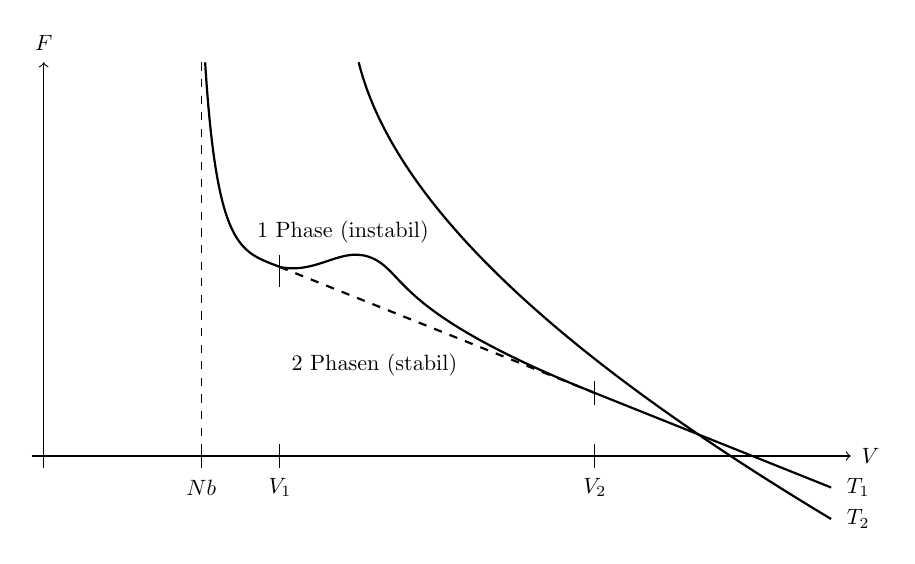
\begin{tikzpicture}[every node/.style = {draw = none, fill = none,scale = 0.8}]
    \draw[->] (0,-0.15) to (0,5);
    \draw[->] (-0.15,0) to (10.25,0);
    \node at (0,5.25) {$F$};
    \node at (10.5,0) {$V$};
    \draw[dashed] (2,5) to (2,0);
    \draw (2,-0.15) to (2,0.15);
    \node at (2,-0.4) {$N b$};
    \draw (3,-0.15) to (3,0.15);
    \node at (3,-0.4) {$V_1$};
    \draw (7,-0.15) to (7,0.15);
    \node at (7,-0.4) {$V_2$};
    \draw[thick] (2.05,5) .. controls (2.2,2.6) and (2.5,2.6) .. (3,2.4) .. controls (3.5,2.3) and (3.8,2.7) .. (4.2,2.5) .. controls (4.6,2.3) and (4.5,1.8) .. (7,0.8) to (10,-0.4);
    \draw[dashed,thick] (3,2.4) to (7,0.8);
    \node[anchor=west] at (10.1,-0.4) {$T_1$};
    \draw[thick] (4,5) .. controls (4.5,3) and (7,1.0) .. (10,-0.8);
    \node[anchor=west] at (10.1,-0.8) {$T_2$};
    \draw (3,2.15) to (3,2.55);
    \draw (7,0.65) to (7,0.95);
    \node[anchor=south] at (3.8,2.6) {1 Phase (instabil)};
    \node[anchor=north] at (4.2,1.4) {2 Phasen (stabil)};
  \end{tikzpicture}
\end{figure}
\begin{tabbing}
\hspace{4em} \= \hspace{4em} \= \kill
$V_1$: $F_1$, flüssig; $V_2$: $F_2$, gasförmig\\
Dazwischen: $V = \alpha V_2 + (1 - \alpha) V_1$, $F = \alpha F_2 + (1 - \alpha) F_1$, da $F$ extensiv!\\
Bestimmung der realen $p(V)$-Kurve: \underline{Maxwell-Konstruktion}\\
2 Phasen in Koexistenz: $\mu_g = \mu_f$, $p_g = p_f$\\
Innerhalb einer Phase: $\mu$ ist (stückweise) eindeutig von $p$,$T$ festgelegt (Gibbs-Duhem)\\
$\rightarrow$\> $\mu(p_2,T) = \mu(p_1,T) + \int\limits_{p_1}^{p_2}\left(\frac{\partial \mu}{\partial p}\right)_{T,N} \dd{p}$ wobei $\mu = \frac{G}{N}$ wegen $G = E - TS + pV$\\
\> $\left(\frac{\partial \mu}{\partial p}\right) = \frac{1}{N} \pdv{G}{p}{T,N} = \frac{V}{N}$ wegen $\dd{G} = -S\dd{T}+V\dd{p}+\mu\dd{N}$\\
\hspace{4em} \= $\mu(p_2,T)$ \= \kill
$\rightarrow$\> $\mu(p_2,T)$ $= \mu(p_1,T) + \frac{1}{N} + \int\limits_{p_1}^{p_2}V \dd{p}$\\
\>\> $= \mu(p_1,T) + \frac{1}{N} + \int\limits_{V_1}^{V_2} V \frac{\dd{p}}{\dd{V}}\dd{p}$\\
\>\> $= \mu(p_1,T) + \frac{1}{N}\left[\left(p_2V_2-p_1V_1\right) -\int\limits_{V_1}^{V_2} p \dd{V}\right]$\\
Gleichgewicht: $p_1=p_2 = \vcentcolon p$, $\mu(p_1,T) = \mu (p_2,T)$\\
$\rightarrow$\> $p(V_1 - V_2) = \int\limits_{V_1}^{V_2}p \dd{V}$ - Interpretation als Fläche im $p$-$V$-Diagramm\\
Druck bei Koexistenz heißt \underline{Dampfdruck}.
\end{tabbing}
\begin{figure}[H]
  \centering
  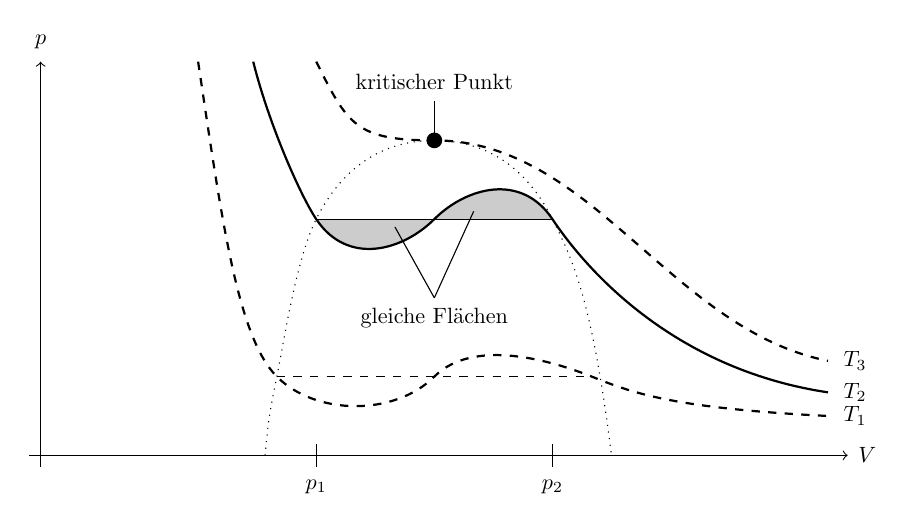
\begin{tikzpicture}[every node/.style = {draw = none, fill = none,scale = 0.8}]
    \draw[->] (-0.15,0) to (10.25,0);
    \draw[->] (0,-0.15) to (0,5);
    \node at (0,5.25) {$p$};
    \node at (10.5,0) {$V$};
    \draw[dotted] (2.85,0) .. controls (2.9,0.5) and (2.9,0.5) .. (3,1) .. controls (3.1,1.5) and (3.25,2.5) .. (3.5,3) .. controls (3.75,3.5) and (4.2,4) .. (5,4) .. controls (5.8,4) and (6.25,3.5) .. (6.5,3) .. controls (6.75,2.5) and (7,2) .. (7.25,0);
    \draw[dashed,thick] (3.5,5) .. controls (3.9,4.2) and (4,4) .. (5,4) .. controls (7,4) and (8,1.6) .. (10,1.2);
    \path[fill=white!80!black] (3.5,3) .. controls (3.9,2.4) and (4.6,2.6) .. (5,3) .. controls (5.4,3.4) and (6.1,3.6) .. (6.5,3);
    \draw[thick] (2.7,5) .. controls (2.9,4.2) and (3.3,3.3) .. (3.5,3) .. controls (3.9,2.4) and (4.6,2.6) .. (5,3) .. controls (5.4,3.4) and (6.1,3.6) .. (6.5,3) .. controls (6.9,2.4) and (8,1.1) .. (10,0.8);
    \draw (3.5,3) to (6.5,3);
    \draw[thick,dashed] (2,5) .. controls (2.3,3) and (2.5,1.5) .. (3.0,1.0) .. controls (3.5,0.5) and (4.5,0.5) .. (5,1) .. controls (5.5,1.5) and (6.5,1.2) .. (7,1) .. controls (7.5,0.8) and (8,0.6) .. (10,0.5);
    \draw[dashed] (3,1) to (7,1);
    \node[anchor=west] at (10.1,1.2) {$T_3$};
    \node[anchor=west] at (10.1,0.8) {$T_2$};
    \node[anchor=west] at (10.1,0.5) {$T_1$};
    \draw (3.5,-0.15) to (3.5,0.15);
    \draw (6.5,-0.15) to (6.5,0.15);
    \node at (3.5,-0.4) {$p_1$};
    \node at (6.5,-0.4) {$p_2$};
    \fill (5,4) circle(0.1);
    \draw (5,4) to (5,4.5);
    \node at (5,4.75) {kritischer Punkt};
    \draw (4.5,2.9) to (5,2);
    \draw (5.5,3.1) to (5,2);
    \node at (5,1.75) {gleiche Flächen};
  \end{tikzpicture}
\end{figure}
\begin{tabbing}
\hspace{4em} \= \hspace{4em} \= \kill
Konstruktion nur möglich unterhalb des kritischen Punkts, $T<T_C$\\
\underline{Bestimmung des kritischen Punkts}:\\
$\left(p + a\frac{N^2}{V^2}\right)(V -N b) = N k_B T\;\;\left|\cdot\frac{V^2}{p}\right.$\\
$\rightarrow$\> $V^3 - \left(N b + \frac{N k_B T}{p}\right)V^2 + a \frac{N^2}{p} V - a b \frac{N^3}{p} = 0$\\
Bei $T = T_C$ stimmen alle drei Nullstellen überein: $\Rightarrow \left(V - V_C\right)^3 = 0$\\
$\rightarrow$\> $V^3 - 3 V_C V^2 + 3 V_C^2 V - V_C^3 = 0$ (Koeffizientenvergleich)\\
(1)\> $3V_C = N b + \frac{N k_B T_C}{p_C}$\\
(2)\> $3V_C^2 = \frac{a}{N^2}{p_C}$\\
(3)\> $V_C^3 = \frac{a b N^3}{p_C}$\\
(3):(2) $\rightarrow$\> $\frac{V_C}{3} = b N$ $\rightarrow$ $V_C = 3 b N$\\
(2) $\rightarrow$\> $p_C = \frac{a N^2}{3\cdot(3 b N)^2} = \frac{a}{27 b^2}$\\
(1) $\rightarrow$\> \fbox{$k_B T_C = \frac{8 a}{27 b}$}\\
Abweichung vom idealen Gas am kritischen Punkt: \fbox{$\frac{p_CV_C}{Nk_BT_C} = \frac{3}{8} = 0.375$} \\
Vergleich mit realen Gasen: Helium $0.31$, Wasser $0.23$\\
Definiere reduzierte, dimensionslose Variablen\\
$p^{*} = \frac{p}{p_C}$, $T^{*} = \frac{T}{T_C}$, $V^{*} = \frac{V}{V_C}$\\
$\rightarrow$\> van der Waals-Gleichung in der Form\\
\> $\left(p^{*}p_C + a \frac{N^2}{V^{*2}V_C^2}\right)(V^{*}V_C - N b) = N k_B T^{*}T_C$\\
\> $\left(p^{*}\frac{a}{27 b^2} + a\frac{N^2}{9 b^2N^2}\frac{1}{V^{*2}}\right)(V^{*}3 b N - N b) = N T^{*} \frac{8 a}{27 b}$\\
$\rightarrow$\> \fbox{$\left(p^{*} + \frac{3}{V^{*2}}\right)(3 V^{*} - 1) = 8 T^{*}$}\\
\underline{Gesetz der korrespondierenden Zustände} - empirisch für viele Gase bestätigt!\\
(Beachte: \= vdW-Gleichung ist ein Spezialfall hiervon, da sie zwei Parameter ($a$, $b$)\\\> und nicht drei ($p_C$, $V_C$, $T_C$) enthält.)\\
\end{tabbing}


\subsection{Van der Waals-Gas am kritischen Punkt}
\begin{tabbing}
\hspace{4em} \= \hspace{4em} \= \kill
Betrachte kleine Abweichungen vom kritischen Punkt:\\
$\Delta p^{*} = p^{*} - 1$, $\Delta T^{*} = T^{*} - 1$, $\Delta V^{*} = V^{*} - 1$\\
$p^{*} = \frac{8 T^{*}}{3V^{*} - 1} - \frac{3}{V^{*2}} = \frac{4 (1 + \Delta T^{*})}{1 + \frac{3}{2}\Delta V^{*}} - \frac{3}{(1 + \Delta V^{*})^2}$\\
Taylor:\>\> $(1 + \frac{3}{2}\Delta V^{*})^{-1} = 1 - \frac{3}{2} \Delta V^{*} + \left(\frac{3}{2} \Delta V^{*}\right)^2 - \left(\frac{3}{2}\Delta V^{*}\right)^3 + \dots$\\
\>\> $(1 + \Delta V^{*})^{-2} = 1 - 2 \Delta V^{*} + 3\Delta V^{*2} - 4 \Delta V^{*3} + \dots$\\
\hspace{4em} \= $p^{*} =$ \= \kill
$\rightarrow$\> $p^{*} =$\> $4 + 4\Delta T^{*} - 3$\\
\>$+ 4\cdot\left(-\frac{3}{2}\Delta V^{*}\right) + 4\Delta T^{*}\left(-\frac{3}{2}\Delta V^{*}\right) + 6\Delta V^{*}$\\
\> $+ 4(1+\Delta T^{*})(\frac{3}{2}\Delta V^{*})^2 - 9\Delta V^{*2}$\\
\> $- 4(1+\Delta T^{*})\cdot(\frac{3}{2}\Delta V^{*})^3 + 12 \Delta V^{*3} + \dots$\\
\> \fbox{$p^{*} = 1 + 4\Delta T^{*} - 6\Delta T^{*}\Delta V^{*} - \frac{3}{2}\Delta V^{*2}$} (antisymmetrisch in $\Delta V^{*}$)\\
$\rightarrow$\> \underline{Kritische Isotherme} ($\Delta T^{*} = 0$): \\
\> $p^{*} = 1 - \frac{3}{2}\Delta V^{*}$
\end{tabbing}
\begin{figure}[H]
  \centering
  \begin{tikzpicture}[every node/.style = {draw = none, fill = none,scale = 0.8},domain=2:8]
    \draw[->] (-0.15,0) to (10.25,0);
    \draw[->] (0,-0.15) to (0,5);
    \node at (0,5.25) {$p^{*}$};
    \node at (10.5,0) {$V^{*}$};
    \draw[thick] plot (\x,{2.5 - 0.09*(\x-5)^3});
    \fill (5,2.5) circle(0.1);
    \draw (5,2.5 ) to (5,2.85);
    \node at (5,3) {Steigung 0};
    \node at (10.15,0.7) {$T = T_C$};
  \end{tikzpicture}
\end{figure}
\begin{tabbing}
\hspace{4em} \= \hspace{4em} \= \kill
\underline{Dampfdruckkurve $p(T)$}: $p_{fl} = p_{gas}$; Maxwell-Konstruktion\\
$\rightarrow$\> $\Delta V^{*}_{fl} = -\Delta V^{*}_{gas}$ wegen Antisymmetrie
\end{tabbing}
\begin{figure}[H]
  \centering
  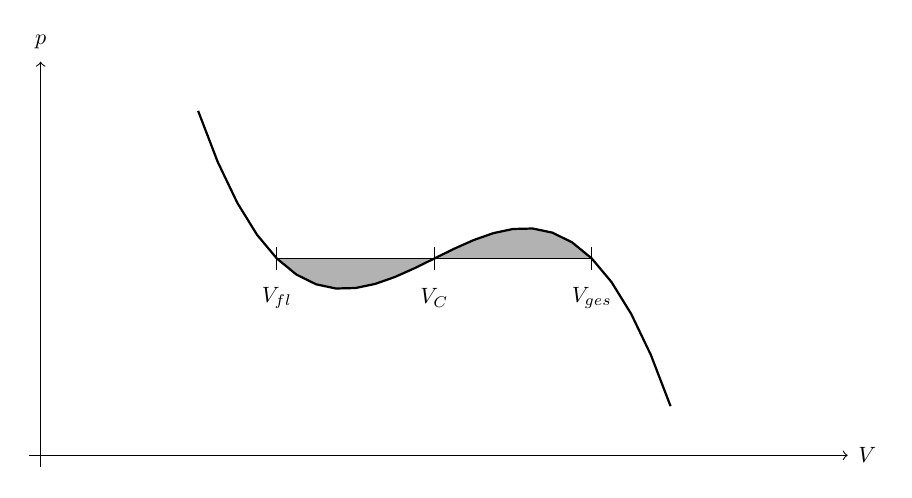
\begin{tikzpicture}[every node/.style = {draw = none, fill = none,scale = 0.8},domain=2:8]
    \draw[->] (-0.15,0) to (10.25,0);
    \draw[->] (0,-0.15) to (0,5);
    \node at (0,5.25) {$p$};
    \node at (10.5,0) {$V$};
    \fill[white!70!black,domain=3:5] plot (\x,{2.5 - 0.125*(\x-5)^3 + 0.5*(\x-5)});
    \fill[white!70!black,domain=5:7] plot (\x,{2.5 - 0.125*(\x-5)^3 + 0.5*(\x-5)});
    \draw[thick] plot (\x,{2.5 - 0.125*(\x-5)^3 + 0.5*(\x-5)});
    \draw (5,2.35) to (5,2.65);
    \draw (7,2.35) to (7,2.65);
    \draw (3,2.35) to (3,2.65);
    \draw (7,2.5) to (3,2.5);
    \node at (3,2) {$V_{fl}$};
    \node at (5,2) {$V_C$};
    \node at (7,2) {$V_{ges}$};
  \end{tikzpicture}
\end{figure}
\begin{tabbing}
\hspace{4em} \= \hspace{4em} \= \kill
$\rightarrow$\> $p_{fl}^{*} = p_{fl}^{*} = p^{*}(\Delta V^{*} = 0) = 1 + 4 \Delta T^{*}$\\
\end{tabbing}
\begin{figure}[H]
  \centering
  \begin{tikzpicture}[every node/.style={draw=none,fill=none,scale=0.8,align=left}]
    \draw[->] (-0.15,0) to (10.25,0);
    \draw[->] (0,-0.15) to (0,5);
    \node at (0,5.25) {$p^{*}$};
    \node at (10.5,0) {$T^{*}$};
    \draw (3,-0.15) to (3,0.15);
    \node at (3,-0.4) {$0$};
    \draw[thick,domain=1:3] plot (\x,4*\x^2/9);
    \draw[dashed] (2,0) to (3,4);
    \fill (3,4) circle (0.1);
    \draw (3.2,3.8) to (3.5,3.8);
    \node[anchor=west] at (3.6,3.8) {Dampfdruckkurve mit\\Steigung 4 am kritischen Punkt};
  \end{tikzpicture}
\end{figure}
\begin{tabbing}
\hspace{4em} \= \hspace{4em} \= \kill
Wegen $p^{*}(\Delta V^{*} = 0) = p^{*}(\Delta V_{fl/gas}^{*})$ gilt: $0 = -6 \Delta T^{*} \Delta V^{*}_{fl/gas} - \frac32\Delta V^{*3}_{fl/gas}$\\
$\rightarrow$\> \fbox{$\Delta V^{*}_{fl/gas} = \pm \sqrt{4\cdot (-\Delta T^{*})}$} Exponent $\frac{1}{2}$
\end{tabbing}
\begin{figure}[H]
  \centering
  \begin{tikzpicture}[every node/.style = {draw = none, fill = none,scale = 0.8}]
    \draw[->] (-0.15,0) to (10.25,0);
    \draw[->] (0,-0.15) to (0,5);
    \node at (0,5.25) {$\Delta V_{fl/gas}$};
    \node at (10.5,0) {$T$};
    \draw (5,-0.15) to (5,0.15);
    \node at (5,-0.4) {$T_C$};
    \draw[thick,domain=2:5] plot (\x,{2*(5-\x)^(1/2)});
    \node[anchor=west] at (5.2,0.4) {$\sim (T_C-T)^{\frac12}$};
  \end{tikzpicture}
\end{figure}
\begin{tabbing}
\hspace{4em} \= \hspace{4em} \= \kill
\underline{Kompressibilität}:\\
Für $T>T_C$:\>\> $\kappa_T = -\frac1V\pdv{V}{p}{T} = -\frac{1}{p_C V^{*}}\pdv{V^{*}}{p^{*}}{T} = -\frac{1}{p_C V^{*}}\pdv{p^{*}}{V^{*}}{T}^{-1}$\\
\> Auf der kritischen Isochore ist $\Delta V^{*} = 0$, $\frac{\partial p^{*}}{\partial V^{*}} = - 6 \Delta T^{*}$\\
$\rightarrow$\> \fbox{$\kappa_T = \frac{1}{6 p_C \Delta T^{*}}$}\\
Für $T< T_C$:\>\> Betrachte Verhalten am Rand des Koexistenzbereichs, das heißt $\Delta V {*} = \Delta^{*}_{fl/gas}$\\
$\rightarrow$\> $\pdv{p^{*}}{V^{*}}{T} = -6 \Delta T^{*} - \frac92 (\Delta V^{*})^2 = 12 \Delta T^{*}$\\
$\rightarrow$\> \fbox{$\kappa_T = \frac{1}{12 p_C}\frac{1}{- \Delta T^{*}}$}\\
\fbox{Bei $T = T_C$ ist $k_T = \infty$. $\rightarrow$ starke Dichteschwankungen. $\rightarrow$ kritische Opaleszenz.}\\
\underline{Schlussfolgerung}: Größen verhalten sich am kritischen Punkt nach Potenzgesetzen mit sogenannten\\
\underline{kritischen Exponenten}\\
\uwave{Beispiel}:\> $\kappa_T\sim |T-T_C|^{-\gamma}$, $T\stackrel{\displaystyle >}{<} T_C$, $\gamma = 1$ für vdW\\
\> $V^{*}_{fl/gas} \sim (T_C-T)^{\beta}$, $T <T_C$, $\beta = \frac12$ für vdW\\
Man findet ein kritisches Verhalten mit systemspezifischen Exponenten in vielen Systemen mit\\ Phasenübergängen. Die Größe $\Delta V^{*}_{fl}$ beziehungsweise $\Delta V^{*}_{gas}$ (oder alternativ Dichteabweichungen $\rho - \rho_C$) kann\\ als \underline{Ordnungsparameter} dienen: eine Größe, die bei $T < T_C$ eine strukturelle Veränderung anzeigt und für\\ $T> T_C$ verschwindet.
\end{tabbing}


\subsection{Ising-Modell (Ferromagnetismus)}
\begin{tabbing}
\hspace{4em} \= \hspace{4em} \= \kill
Nichtwechselwirkende Spins $\vec{s}_j$ im Magnetfeld $\vec{B}$:\\
\> $H = -\sum\limits_j \vec{\mu}_j\cdot \vec{B}$ mit magnetischen Momenten $\vec{\mu}_j = -g \frac{\mu_B}{\hbar} \vec{s}_j$ (für einfach negativ geladene Teilchen)\\
\> $\mu_B = \frac{e \hbar}{2 m_e} =$ Bohrsches Magneton\\
\> $g = 2$ (Annahme Elektron)\\
$\rightarrow$\> $H = 2 \frac{\mu_B}{\hbar}\sum\limits_j \vec{s}_j\cdot\vec{B} = \mu_B \sum\limits_j \vec{\sigma}_j\cdot\vec{B}$ mit Pauli-Vektoren $\vec{\sigma}_j$\\
Betrachte jetzt zusätzlich Wechselwirkung benachbarter Spins (Annahme, dass Spins auf einem regelmäßigen\\ Gitter platziert sind).\\
$\rightarrow$\> $H = 2 \frac{\mu_B}{\hbar} \sum\limits_j \vec{s}_j \cdot \vec{B} - I\cdot\sum\limits_{\{j,l\}} \vec{s}_j\cdot \vec{s}_l$ \underline{Heisenberg-Modell}\\
$\sum\limits_{\{j,l\}}$ ist Summe über benachbarte Paare\\
$I > 0$:\> parallele Spins energetisch bevorzugt $\rightarrow$ Ferromagnet\\
$I < 0$:\> antiparallele Spins energetisch bevorzugt $\rightarrow$ Anttiforromagnet\\
Vereinfachtes Modell: Ersetze $\vec{s}_j\cdot \vec{s}_l$ $\rightarrow$ $s_{j,z}\cdot s_{l,z}$ \underline{Ising-Modell} (nur z-Komponenten) und $\vec{B} = B \vec{e}_z$\\
Vereinfachte Notation: \fbox{$H = B \sum\limits_j S_j - J \sum\limits_{\{j,l\}}S_jS_l$}, $S_j = \pm 1$\\
$\left\langle\sum\limits_j S_j\right\rangle = M =$ \glqq Magnetisierung\grqq (eigentlich: $M =\frac{\text{gesamtes magnetisches Moment}}{\mu_B}$).\\
\underline{1-dimensionales Ising-Modell}: $H = B\sum\limits_{j=1}^{N} - J\sum\limits_{j=1}^{N} S_j S_{j+1}$\\
(mit periodischen Randbedingungen: $S_{N+1} = S_1$)\\
Zustandssumme: $Z = \sum\limits_{S_1}\dots\sum\limits_{S_N} e^{-\beta H} = \sum\limits_{S_1} \dots\sum\limits_{S_N}\prod\limits_{j=1}^{N} \exp\left(-\frac{b}{2}(S_j + S_{j+1}) + K S_jS_{j+1}\right)$\\
\> $b = \beta B$, $K = \beta J$\\
\underline{Lösung mit Transfermatrix-Methode}:\\
Definiere \underline{Transfermatrix} $T = \left(\begin{array}{c c} e^{K-b}& e^{-K}\\ e^{-K} & e^{K + b}\end{array}\right) = \left(\begin{array}{c c} T_{1,1} & T_{1,-1}\\ T_{-1,1} & T_{-1,-1}\end{array}\right)$\\
$\rightarrow$\> $T_{S,S'} = \exp \left(-\frac{b}{2} (S + S') + K S S'\right)$\\
$\rightarrow$\> $Z = \sum\limits_{S_1} \dots\sum\limits_{S_N} \prod\limits_{j=1}^{N} T_{S_j,S_{j+1}} = \sum\limits_{S_1} (T^N)_{S_1,S_N+1} = \spur\left(T^N\right)$\\
Berechnung der Spur:\\
\> Zunächst Eigenwerte $\lambda$ von $T$, $(e^{K - b} - \lambda)(e^{K+b} - \lambda) - e^{-2K} = 0$\\
\> $\lambda^2 - 2\lambda e^{K} \cosh (b) + e^{2K} - e^{-2K}$ $\lambda_{1,2} = e^{K} \cosh (b) \pm \sqrt{e^{-2K} + e^{2K}\sinh ^{2}(b)}$.\\
Eigenwerte von $T^N$: $\lambda_{1,2}^N$ $\rightarrow$ $\spur \left(T^N\right) = \lambda_1^N + \lambda_2^N$\\
Freie Energie: $F = -k_B T \ln Z = - k_B T \ln \left(\lambda_1^N + \lambda_2^N\right)$\\
Sei $\lambda_1$ der größere Eigenwert. $F = - k_B T N \ln\left[\lambda_1\cdot\left(1+\left(\frac{\lambda_2}{\lambda_1}\right)^N\right)^{\frac{1}{N}}\right]$\\
\> $1 + \left(\frac{\lambda_2}{\lambda_1}\right)^N \stackrel[N\to\infty]{}{\longrightarrow} 1$\\
$\rightarrow$\> $F = - k_B T \ln \lambda_1$\\
Bei $B = 0$: $F = - k_B T N \ln\left(2 \cosh\frac{J}{k_B T}\right)$\\
$\dd{F} = -S\dd{T} - \mu\dd{B}$ $\rightarrow$ $S = -\pdv{F}{T}{B}$, $C_B= T \pdv{S}{T}{B} = - T \npdv{F}{T}{B}{2}$\\
$\rightarrow$\> \underline{glattes Verhalten}, \underline{kein Phasenübergang}
\end{tabbing}
\begin{figure}[H]
  \centering
  \begin{tikzpicture}[every node/.style={draw=none,fill=none,scale=0.8,align=left}]
    \draw[->] (-0.15,0) to (10.25,0);
    \draw[->] (0,-0.15) to (0,5);
    \node at (0,5.25) {$C_{B=0}$};
    \node at (10.5,0) {$T$};
    \draw[thick,domain=0.4:1] plot (\x,{40/(cosh(2/\x))^2/\x^2)});
    \draw[thick,domain=1:2]   plot (\x,{40/(cosh(2/\x))^2/\x^2)});
    \draw[thick,domain=2:3]   plot (\x,{40/(cosh(2/\x))^2/\x^2)});
    \draw[thick,domain=3:5]   plot (\x,{40/(cosh(2/\x))^2/\x^2)});
    \draw[thick,domain=5:10]  plot (\x,{40/(cosh(2/\x))^2/\x^2)});
  \end{tikzpicture}
\end{figure}
\begin{tabbing}
\hspace{4em} \= \hspace{4em} \= \kill
\underline{2-dimensionales Ising-Modell} (Quadratgitter)\\
-- Exakte Lösung möglich (Onsager 1944)\\
-- Man findet Unstetigkeit der Wärmekapazität bei kritischer Temperatur (\underline{Phasenübergang})\\
-- Für $J > 0$, $B = 0$: \= $T < T_C$ $\rightarrow$ \underline{spontane Symmetriebrechung}: Magnetisierung $\neq 0$, \underline{Ferromagnet}\\
\> $T>T_C$ $\rightarrow$ Magnetisierung $=0$, \underline{Paramagnet}\\
Ordnungsparameter: spontane Magnetisierung (Maß für ferromagnetische Ordnung)\\
-- \= Bei $T<T_C$ herrscht \underline{langreichweitige Ordnung}.\\
\> Korrelationslänge $\chi$ in $\left\langle\left(S_{\vec{r}} - \left\langle S_{\vec{r}}\right\rangle\right)\left(S_{\vec{r}'} - \left\langle S_{\vec{r}'}\right\rangle\right)\right\rangle \sim e^{-\frac{|\vec{r} - \vec{r}'}{\chi}}$ divergiert.\\
-- In der Nähe von $T_C$: kritische Exponenten für \= Magnetisierung $M$\\
\> Wärmekapazität $C_B$\\
\> Suszeptibilität $\chi_T = \pdv{M}{B}{T}$
\end{tabbing}


\subsection{Klassifizierung von Phasenübergängen}
\begin{tabbing}
\hspace{4em} \= \hspace{4em} \= \kill
Phasenübergang $=$\\
\>Umwandlung einer Phase in eine andere beziehungsweise Gemisch aus koexistierenden Phasen\\
\underline{Klassifizierung nach Ehrenfest}:\\
Übergang der Ordnung n $\stackrel{\wedge}{=}$ \= -- n. Ableitung des relevanten thermodynamischen Potentials \underline{unstetig}\\
\> -- Ableitungen niedrigerer Ordnung \underline{stetig}\\
Übergänge, die nicht 1. Ordnung sind, aber dennoch eine Singularität der Wärmekapazität zeigen,\\ heißen \underline{$\lambda$-Übergänge}:
\end{tabbing}
\begin{figure}[H]
  \centering
  \begin{tikzpicture}[every node/.style={draw=none,fill=none,scale=0.8,align=left}]
    \draw[->] (-0.15,0) to (10.25,0);
    \draw[->] (0,-0.15) to (0,5);
    \node at (0,5.25) {$C$};
    \node at (10.5,0) {$T$};
    \draw (5,-0.15) to (5,0.15);
    \draw[dashed] (5,0) to (5,5);
    \node at (5,-0.4) {$T_C$};
    \draw[thick,domain=0:4] plot (\x,{1/((5-\x))});
    \draw[thick,domain=4:4.8] plot (\x,{1/((5-\x))});
    \draw[thick,domain=5.2:6] plot (\x,{1/(5*(\x-5)^2)});
    \draw[thick,domain=6:10] plot (\x,{1/(5*(\x-5)^2)});
  \end{tikzpicture}
\end{figure}
\begin{table}[H]
  \centering
  \begin{tabular}{c || c | c | c | c}
    Übergang & \begin{tabular}{c} vdW ($T<T_C$) \\ flüssig $\to$ gasförmig \end{tabular} & \begin{tabular}{c}vdW\\$T>T_C$ $\to$ $T<T_C$\end{tabular} &\begin{tabular}{c} Ising\\$T>T_C$ $\to$ $T<T_C$\end{tabular} & BEC \\\hline\hline
    \begin{tabular}{c}Ordnung\\ (Ehrenfest)\end{tabular} & 1 & 2 & 2 ($\lambda$) & 3 (nicht wechselwirkend) \\\hline
    \begin{tabular}{c}Ordnungs-\\parameter\end{tabular} & $\Delta \rho = \rho - \rho_C$ & $\Delta \rho$ & $M$ & \begin{tabular}{c}makroskopische\\Wellenfunktion\\(komplex)\end{tabular} \\\hline
    \begin{tabular}{c}gebrochene\\Symmetrie\end{tabular} & -- & \glqq Reflexion\grqq & $S_Z$ $\to$ $-S_Z$ &\begin{tabular}{c}Eichsymmetrie\\(der globalen Phase)\end{tabular} \\\hline
    \begin{tabular}{c}unstetige\\Größe(n)\end{tabular} & \begin{tabular}{c}Entropie $S$\\ Volumen $V$\\ Dichte $\rho$ \end{tabular} & $C_V$ & $C_B$ & $\frac{\partial C_V}{\partial T}$ \\\hline
     & & \multicolumn{3}{|c}{Ordnungsparameter stetig}
  \end{tabular}
\end{table}
\begin{tabbing}
\underline{Moderne Einteilung}: \= 1. Ordnung $\stackrel{\wedge}{=}$ Ordnungsparameter unstetig\\
\> 2. Ordnung $\stackrel{\wedge}{=}$ Ordnungsparameter stetig
\end{tabbing}


\subsection{Kritische Exponenten}
\begin{tabbing}
\hspace{4em} \= \kill
In der Nähe der kritischen Temperatur $T_C$ gilt ($t = \frac{T-T_C}{T_C}$):\\
\> Wärmekapazität: $C \propto |t|^{-\alpha}$\\
\> Ordnungsparameter: $\psi \propto |t|^{\beta}$\\
\> Suszeptibilität/ Kompressibilität: $\chi \propto |t|^{-\gamma}$\\
\> Korrelationslänge: $\xi \propto |t|^{-\nu}$\\
Aus der Annahme von Potenzgesetzen lässt sich herleiten:\\
\> $\alpha =\alpha'$, $\gamma = \gamma'$, $\nu = \nu'$ (gleiche Exponenten ober-/unterhalb $T_C$)\\
\fbox{$\alpha + 2\beta + \gamma = 2$, $2 - \alpha = d\cdot \nu$} in $d$ Dimensionen (\underline{Skalengesetze})
\end{tabbing}
